\documentclass[9pt]{extarticle}

\usepackage[margin=0.64in]{geometry}
\usepackage{amsmath,amssymb,amsthm,mathtools}
\usepackage{booktabs}
\usepackage{array}
\newcolumntype{L}[1]{>{\raggedright\arraybackslash}p{#1}}
\usepackage{enumitem}
\usepackage{hyperref}
\usepackage{microtype}
\usepackage{tikz}
\usetikzlibrary{arrows.meta,positioning,calc,fit}

\hypersetup{colorlinks=true,linkcolor=blue,urlcolor=blue,pdftitle={ZenoDEX: Full-System Architecture and Public Assurance Boundary},pdfauthor={Dana Edwards}}
\setlist[enumerate]{nosep,leftmargin=5mm}
\setlength{\textfloatsep}{8pt plus 1pt minus 2pt}
\setlength{\floatsep}{8pt plus 1pt minus 2pt}
\setlength{\intextsep}{8pt plus 1pt minus 2pt}
\setlength{\abovedisplayskip}{7pt}
\setlength{\belowdisplayskip}{7pt}
\setlength{\abovecaptionskip}{4pt}
\setlength{\belowcaptionskip}{0pt}

\newcommand{\Exec}{\mathsf{Exec}}
\newcommand{\Guards}{\mathsf{Guards}}
\newcommand{\Cert}{\mathsf{Cert}}
\newcommand{\Runtime}{\mathsf{Runtime}}
\newcommand{\Assure}{\mathsf{Assure}}
\newcommand{\Key}{\mathsf{Key}}
\newcommand{\Winner}{\mathsf{Winner}}
\newcommand{\argmin}{\operatorname*{arg\,min}}
\newcommand{\code}[1]{\path{#1}}

\newtheorem{claim}{Claim}

\title{ZenoDEX: Full-System Architecture and Public Assurance Boundary}
\author{Dana Edwards}
\date{April 2026}

\begin{document}
\maketitle

\begin{abstract}
ZenoDEX is intended to be a proof-carrying exchange architecture, not only a
spot DEX runtime. The whole system spans theorem-bearing spot kernels,
fail-closed guard planes, certificate-carrying settlement and price surfaces,
bounded stablecoin and perpetual-risk layers, narrow replayable runtime
adapters, and a public assurance boundary that is deliberately narrower than the
full target architecture. This short paper states that whole-system thesis and
makes the current public claim boundary explicit.
\end{abstract}

\paragraph{Contributions.}
This paper contributes:
\begin{enumerate}
  \item a compact whole-system decomposition;
  \item a public-safe evidence discipline;
  \item a guarantee-and-assumption summary for the main surfaces;
  \item an explicit separation between the full architecture and the current
  RC1 release claim.
\end{enumerate}

\section{Whole-system thesis}
The intended architecture is
\[
\mathsf{ZenoDEX}
:= \Exec \wedge \Guards \wedge \Cert \wedge \mathsf{Control}
\wedge \mathsf{Oracle} \wedge \mathsf{zUSD} \wedge \mathsf{Perps}
\wedge \Runtime \wedge \Assure.
\]
Standard reading: the whole system includes execution, guards, certificates,
risk layers, runtime adapters, and assurance surfaces.
Practical consequence: the correct review object is the architecture, not one
isolated module.

The current public discipline is
\[
\mathsf{PublicClaim} \subset \mathsf{EvidenceFrontier} \subset \mathsf{FullTargetArchitecture}.
\]
Standard reading: the current release claim is narrower than the strongest
public evidence, and both are narrower than the intended full system.
Practical consequence: an honest paper may describe the full stack while still
keeping the release claim conservative.

\begin{figure}[t]
\centering
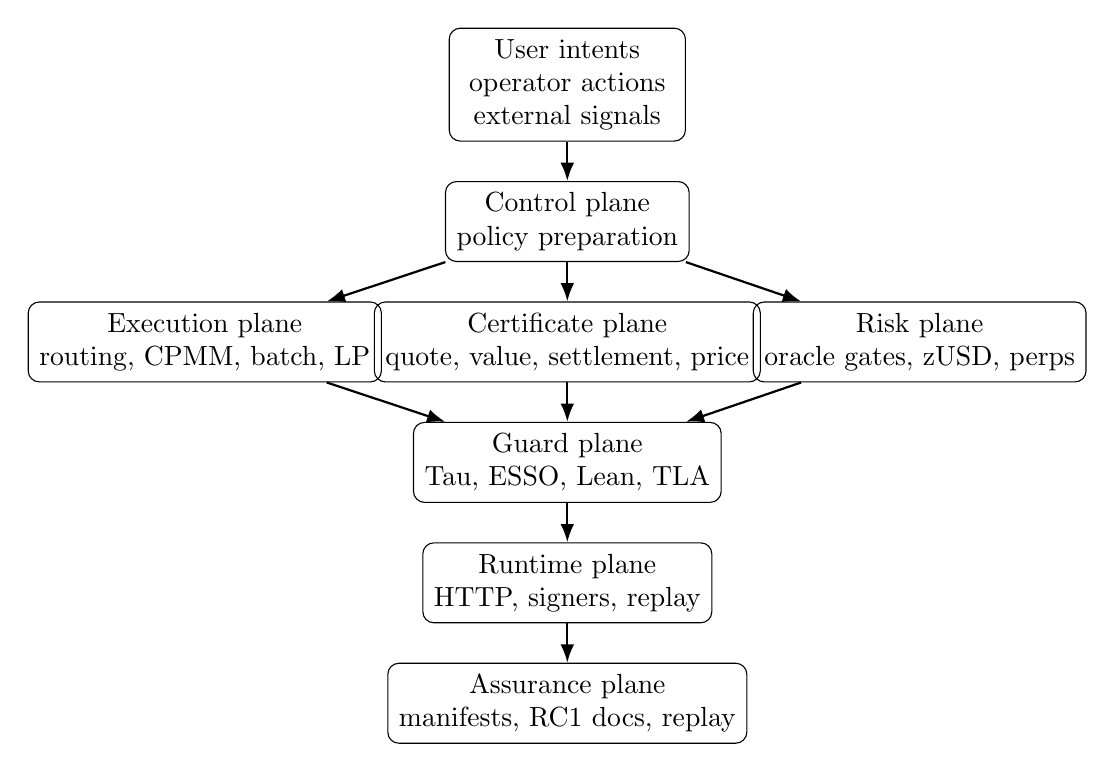
\begin{tikzpicture}[
  node distance=5mm and 8mm,
  box/.style={draw, rounded corners, align=center, inner sep=4pt, minimum width=30mm},
  arr/.style={-Latex, thick}
]
\node[box] (intent) {User intents\\operator actions\\external signals};
\node[box, below=of intent] (control) {Control plane\\policy preparation};
\node[box, below left=of control] (exec) {Execution plane\\routing, CPMM, batch, LP};
\node[box, below=of control] (settle) {Certificate plane\\quote, value, settlement, price};
\node[box, below right=of control] (risk) {Risk plane\\oracle gates, zUSD, perps};
\node[box, below=of settle] (guards) {Guard plane\\Tau, ESSO, Lean, TLA};
\node[box, below=of guards] (runtime) {Runtime plane\\HTTP, signers, replay};
\node[box, below=of runtime] (assure) {Assurance plane\\manifests, RC1 docs, replay};
\draw[arr] (intent) -- (control);
\draw[arr] (control) -- (exec);
\draw[arr] (control) -- (settle);
\draw[arr] (control) -- (risk);
\draw[arr] (exec) -- (guards);
\draw[arr] (settle) -- (guards);
\draw[arr] (risk) -- (guards);
\draw[arr] (guards) -- (runtime);
\draw[arr] (runtime) -- (assure);
\end{tikzpicture}
\caption{Whole-system stack. Advisory or planning surfaces may influence preparation, but execution authority flows only through fail-closed guards and narrow runtime adapters.}
\end{figure}

\section{Evidence rule}
The governing evidence order is
\[
\mathtt{proved} > \mathtt{contract} > \mathtt{implemented} > \mathtt{replay\_backed} > \mathtt{hypothesis}.
\]
Standard reading: every claim is limited by the strongest public replayable
support actually present.
Practical consequence: theorem-bearing spot slices, packet contracts, and
release gates are intentionally not collapsed into one generic label.

\section{Execution and certificate planes}
The canonical execution pattern is
\[
\Winner(C) := \argmin_{c \in C} \Key(c),
\]
with certificate-bearing settlement shaped by
\[
\mathsf{SettlementOK} \to \mathsf{CanonicalDeltaTable} \wedge \mathsf{ReplayVerifiable}.
\]
Standard reading: bounded candidate families are resolved by explicit total
keys, and accepted settlement must carry replay-checkable canonical meaning.
Practical consequence: determinism is treated as semantic canonicality plus
replayable packet structure, not only as stable iteration order.

The strongest public theorem stock today lives in the spot execution plane:
\begin{itemize}
  \item canonical batch winner theorems,
  \item exact-in winner and packet shells,
  \item CPMM invariant and accounting theorems,
  \item fee-dust carry and anti-fragmentation helper theorems.
\end{itemize}
The certificate plane then lifts these local mechanisms into public packet and
settlement surfaces.

\section{Control, oracle, and runtime planes}
The full system is not only math plus packets. The admission layer is
\[
\mathsf{AdmittedIntent}
:= \mathsf{NormalFormOK} \wedge \mathsf{SignatureOrWitnessOK}
\wedge \mathsf{NonceOK} \wedge \mathsf{BoundaryContractOK},
\]
and the price-admission layer is
\[
\mathsf{PriceInputAccepted}
\to \mathsf{FreshnessBound} \wedge \mathsf{PendingStateConsistent}
\wedge \mathsf{ProvenancePacketCoherent}.
\]
Standard reading: the runtime only becomes authoritative after normalization,
authentication, nonce discipline, and oracle/provenance checks succeed.
Practical consequence: the public system claim must include ingress and price
discipline, not only the inner execution kernels.

The supported runtime path is still narrower than the whole repository:
\[
\mathsf{SupportedHTTP} \subset \mathsf{AllRuntimeEndpoints}.
\]
Practical consequence: the paper describes the whole runtime stack, but the
release claim stays bounded to the documented supported boundary.

\section{Risk and runtime planes}
The runtime path is narrower than the full repository:
\[
\mathsf{SupportedHTTP} \subset \mathsf{AllRuntimeEndpoints}.
\]
The monetary and derivatives layers are also narrower than the end-state target.
Representative public formulas are:
\[
\mathsf{zUSDAdmissible} \to \mathsf{DebtConservation} \wedge \mathsf{CollateralConservation},
\]
\[
\mathsf{PerpTransitionAllowed} \to \mathsf{FreshOracleWindow} \wedge \mathsf{BoundedMoveGate}.
\]
Standard reading: zUSD and perps are covered by explicit bounded public safety
claims, not by a blanket claim that the whole risk stack is fully proved.
Practical consequence: the full system is covered in the architecture, but the
public release claim remains more conservative than the target design.

\section{Assurance plane}
The public assurance plane is executable:
\[
\mathsf{PublishedClaimOK}
\to \mathsf{ManifestPinned} \wedge \mathsf{ReplaySurfaceTracked}
\wedge \mathsf{GeneratedEvidenceRebuildable}.
\]
Standard reading: the release claim is only meaningful if the public replay
lanes and manifests remain synchronized.
Practical consequence: the repo's assurance documents are part of the system,
not only documentation about it.

\section{RC1 public boundary}
The current public RC1 contract is
\[
\mathsf{RC1ClaimOK} := \mathsf{CleanTree} \wedge \mathsf{ScopeFrozen} \wedge \mathsf{ReplayGreen} \wedge \mathsf{ExclusionsHonest}.
\]
Standard reading: the RC1 claim is configuration-specific, replay-backed, and
explicitly bounded.
Practical consequence: the public release claim is narrower than the whole
architecture described in this paper.

\begin{table}[t]
\centering
\small
\begin{tabular}{@{}L{31mm}L{23mm}L{27mm}L{53mm}@{}}
\toprule
Surface & Intended guarantee & Current strongest public evidence & Main limit \\
\midrule
Spot execution & canonical bounded winner relation & proved & bounded emitted candidate domain \\
Settlement / quote binding & replayable canonical packet surfaces & contract + tests + proved helper shells & packet semantics still depend on explicit admission contracts \\
Runtime ingress & signer / nonce / receipt discipline & contract + tests & supported HTTP subset is intentionally narrow \\
zUSD / oracle safety & bounded solvency and stale-oracle fail-closed posture & mixed & not every stablecoin claim is release-backed \\
Perps / funding / liquidation & bounded risk-envelope posture & mixed & not a blanket derivatives-complete proof \\
RC1 public release & replayable public assurance surface & contract + replay evidence & clean tree and honest exclusions required \\
\bottomrule
\end{tabular}
\caption{Compact guarantee matrix.}
\end{table}

\section{End-state proof agenda}
The remaining agenda is to widen bounded canonicality into broader packet and
generator surfaces, strengthen zUSD and perps from mixed public posture toward
stronger theorem-backed claims, and keep runtime replay boundaries aligned with
the same canonical payload semantics enforced below them.

This paper is grounded only in public-safe artifacts:
\begin{itemize}
  \item \code{docs/PUBLIC_ASSURANCE_REPLAY.md}
  \item \code{docs/RC1_SCOPE.md}
  \item \code{docs/RC1_VERIFIED_SURFACE_MATRIX.md}
  \item \code{docs/TLA_CLAIM_SUMMARY.md}
  \item \code{docs/claims_registry.yaml}
  \item theorem-bearing files under \code{lean-mathlib/Proofs/}
  \item public kernels under \code{src/kernels/dex/}
\end{itemize}

\end{document}
